\section{Deep Gated Networks (DGN): Information Flow via Sub-Networks}\label{sec:pathgate}
In what follows, we denote the dataset by $(x_s,y_s)_{s=1}^n\in\R^{d_{in}}\times \R$. A DGN is given by:
\FloatBarrier
\begin{table}[h]
\begin{minipage}{0.5\columnwidth}
\resizebox{\columnwidth}{!}{
\begin{tabular}{|l|l|}\hline
\multicolumn{2}{|c|}{Value Network: $\N(\Theta_t;\G_t)$}\\\hline 
Input layer & $z_{x,\Theta_t}(0)=x$ \\\hline
Pre-activation & $q_{x,\Theta_t}(l)={\Theta_t(l)}^\top z_{x,\Theta_t}(l-1)$\\\hline
Layer output & $z_{x,\Theta_t}(l)=q_{x,\Theta_t}(l)\odot G_{x,t}(l)$ \\\hline
Final output & $\hat{y}_t(x)={\Theta_t(d)}^\top z_{x,\Theta_t}(d-1)$\\\hline
Gating Values& $\begin{aligned}\G_t\stackrel{def}=\{G_{x_{s},t}(l,i), \forall s\in[n],\\l\in[d-1],i\in[w]\}\end{aligned}$\\\hline
\end{tabular}
}
\end{minipage}
\begin{minipage}{0.5\columnwidth}
\resizebox{\columnwidth}{!}{
\begin{tabular}{|c|c|}\hline
Gating Network: $\G(\Tg_t,\beta)$\\\hline
$z_{x,\Tg_t}(0)=x$  \\\hline
$q_{x,\Tg_t}(l)={\Tg_t(l)}^\top z_{x,\Tg_t}(l-1)$ \\\hline
$z_{x,\Tg_t}(l)=q_{x,\Tg_t}(l)\odot G_{x,\Tg_t}(l)$ \\\hline
{$\begin{aligned}\beta >0: G_{x,\Tg_t}(l,i)&=\frac{1+\epsilon}{1+\exp(-\beta q_{x,\Tg_t}(l,i))} \\ \beta=\infty: G_{x,\Tg_t}(l,i)&=\mathbbm{1}_{\{q_{x,\Tg_t}(l,i)>0\}}\end{aligned}$}\\\hline 
\end{tabular}
}
\end{minipage}
\caption{Here $\Theta(l,i,j)$ denotes the weight connecting node $i$ of layer $l-1$ to node $j$ of layer $l$, and $\odot$ stands for the \emph{Hadamard} product. $q(l),z(l)$ and $G(l)$ are $w$-dimensional quantities. The left table shows the value network, and the right table shows the gating network.  At time $t$, by specifying the gating values for all the $n$ input examples as $\G_t\stackrel{def}=\{G_{x_{s},t}(l,i), \forall s\in[n],l\in[d-1],i\in[w]\}$, we can recover the outputs $\hat{y}_t(x_s)\in \R$ for all the inputs $\{x_s\}_{s=1}^n$ in the dataset. We denote a DNG by $\N(\Theta_t;\G(\Tg_t,\beta)$ or simply $\N(\Theta_t;\Tg_t,\beta)$.}
\label{tb:dgn}
\end{table}
We consider fully connected deep networks with $d$ layers, and $w$ hidden units per layer. We have a total of $P=d_{in}w^{(d-1)}$ paths. Let us say that an enumeration of the paths is given by $[P]=\{1,\ldots,P\}$. Let $\I_{l}\colon [P]\ra [w],l=0,\ldots,d-1$ provide the index of the hidden unit through which a path $p$ passes in layer $l$ (with the convention that $\I_d(p)=1,\forall p\in [P]$). We can then define: i) the value of a path $p$ by $v_t(p)\stackrel{def}=\Pi_{l=1}^d \Theta_t(l,\I_{l-1}(p),\I_l(p))$ and ii) the activity of a path $p$ for an input $x_s\in \R^{d_{in}}$ by $A_{t}(x,p)\stackrel{def}{=}\Pi_{l=1}^{d-1} G_{x_s,t}(l,\I_l(p))$.\\
 The \emph{neural path feature (NPF)} of an input example $x_s\in \R^{d_{in}}$ is given by $\phi_{x_s,\G_t}=(x_s(\I_0(p))A_t(x_s,p) ,p\in[P])\in\R^P$. Here, for a path $p$, $\I_0(p)$ is the input node at which the path starts, and $A_t(x_s,p)$ is its activity. By arranging the NPF of the $n$ input examples in a matrix $\Phi_t=(\phi_{x_s,\G_t},s\in[n])\in\R^{P\times n}$, we can express the predicted output of a DGN as: 
\begin{align}\label{eq:npfbasic}
\hat{y}_t=\Phi_t^\top v_t,
\end{align}
where, the value of the path $v_t$ is the equivalent of the so called \emph{weight-vector} in a standard linear approximation. The \emph{neural path kernel} (NPK) matrix is defined as $H_t\stackrel{def}=\Phi^\top_t\Phi_t$. The information flow in a DGN has the following interesting properties.\\
\begin{figure*}[t]
%\begin{minipage}{0.78\columnwidth}
\resizebox{\columnwidth}{!}{
\begin{tabular}{ccc}
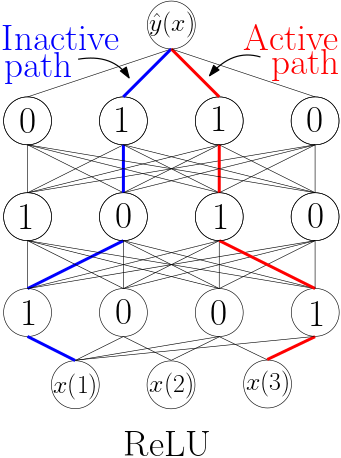
\includegraphics[scale=0.5]{figs/nn.png}
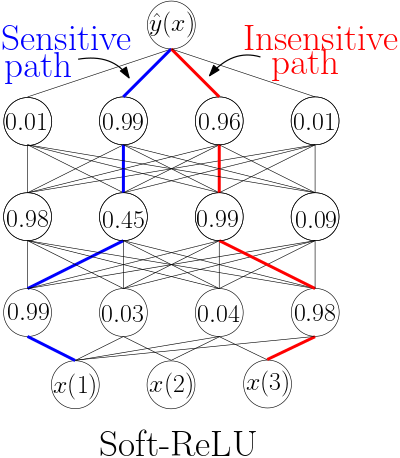
\includegraphics[scale=0.5]{figs/nnsoft.png}
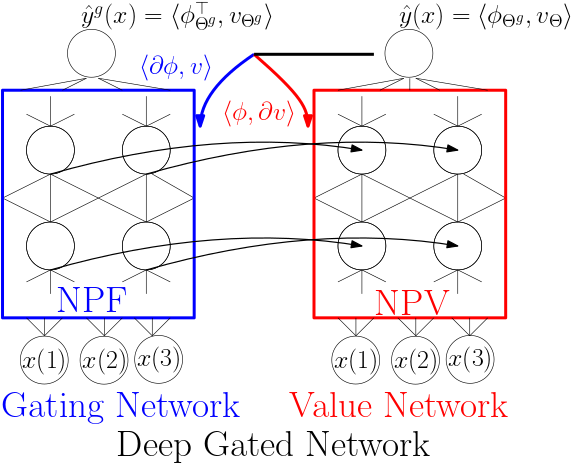
\includegraphics[scale=0.5]{figs/nntwin-blck.png}
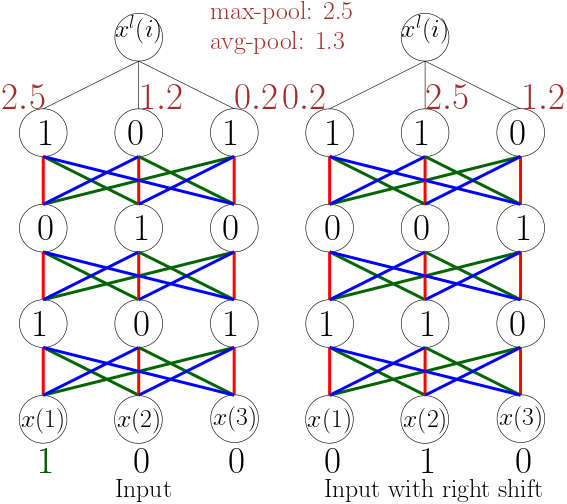
\includegraphics[scale=0.5]{figs/nnconv.png}
%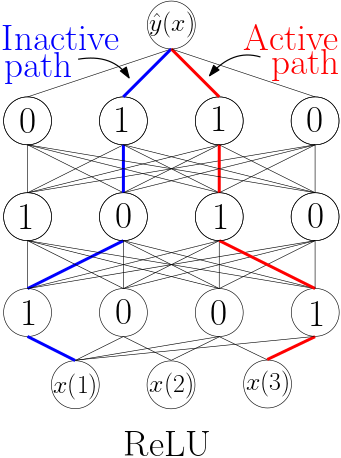
\includegraphics[scale=0.5]{figs/nn.png}
%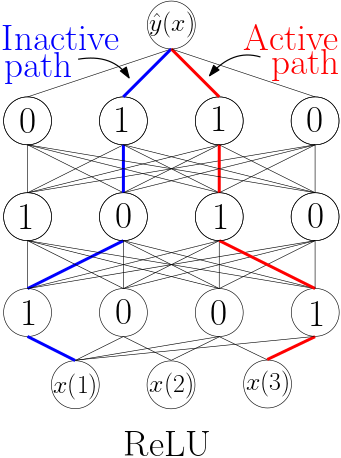
\includegraphics[scale=0.5]{figs/nn.png}
\end{tabular}
}
%\end{minipage}
%\begin{minipage}{0.18\columnwidth}
%\resizebox{\columnwidth}{!}{
%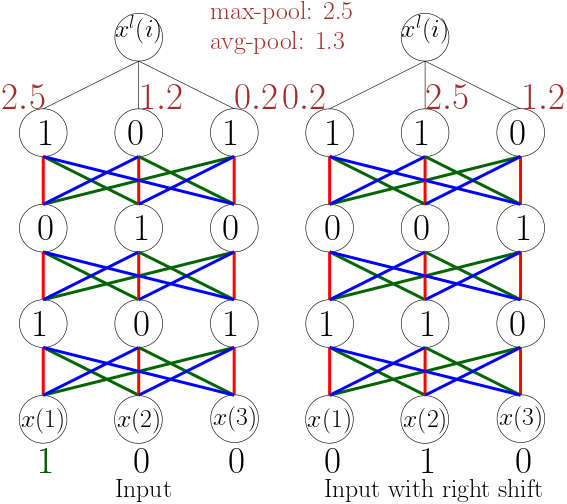
\includegraphics[scale=0.5]{figs/nnconv.png}
%}
%\end{minipage}
\caption{Cartoon illustration of usefulness of path-view and DGN framework.}
\label{fig:cartoon}
\end{figure*}
$1.$ \textbf{Representational Power:} The ability of DNNs to fit data has been demonstrated in the past. \cite{ben} showed that DNNs can fit even random labels, and random pixels of standard datasets such as MNIST. However, we note that, for standard DNNs with ReLU gates, with no bias parameters, a dataset with $n=2$ points namely $(x,1)$ and $(2x,-1)$ for some $x\in \R^{d_{in}}$ cannot be memorised. The reason is that the gating values are the same for both $x$ and $2x$ (for that matter any positive scaling of $x$), and hence $\phi_{2x,\G_t }= 2\phi_{x,\G_t }$, and thus it not possible to fit arbitrary values for $\hat{y}_t(x)$ and $\hat{y}_t(2x)$.\\
$2.$ \textbf{Translation Invariance:} Consider a convolution network using $l$ layers of circular convolutions\footnote{Here, instead of zero-padding in the corners, we follow the convention that index $d_{in}+k$ will be interpreted as $k$, for $k>0$, and $-k$ will be interpreted as $d_{in}-k$.} with filter size $k'<d_{in}$ and unit stride, and let $x^l(i)$ be the output of the $i^{th}$ channel after either $\max$-/global average-pooling. Looking at the right most illustration in \Cref{fig:cartoon}, it is easy to check translation invariance property: the red, blue, green lines illustrate that circular symmetry in the path values, due to which, a translation in the input will cause all the internal variable to translate, and final invariance results from the invariance of the $\max$/average operation.\\
$3.$ \textbf{Twin Gradients:} The derivate of the output $\partial \hat{y}$ has two components, i) the \emph{value derivative} given by $(\partial v)^\top \phi$ and ii) the \emph{feature derivative} given by $(\partial \phi)^\top v$.\\
$4.$ \textbf{Hard Gate/ReLU artefact:} Note that when the gating values belong to $\{0,1\}$ (as with the case of ReLU activations), the feature derivative given by $(\partial \phi)^\top v =\sum_{p\in[P]}x(\I_0(p))\partial A(x,p) v(p)$ is $0$. However, in a network with ReLU activations the gating values and hence the path activities $A_t(\cdot,\cdot)$ changes during training. We fix this artefact arising due to non-differentiability by considering \emph{soft-gates}, see the $\beta>0$ case in \Cref{tb:dgn}. The difference between hard and soft gates can be seen in the first two illustrations in \Cref{fig:cartoon}, where negative/positive values lead to $0/1$ in the case of hard gating, and close to $0/1$ in the case of soft-gating.\\
$5.$ \textbf{Active/Sensitive sub-networks:} The value derivative/gradient flows through the set active paths. To see this, note that $(\partial v)^\top \phi=\sum_{p\in[P]}x(\I_0(p))A(x,p)\partial v$, i.e., only paths $p$ with $A(x,p)$ close to $1$ contribute to the summation. The feature derivative/gradient flows through the set of sensitive paths. To see this, note that $(\partial \phi)^\top v =\sum_{p\in[P]}x(\I_0(p))\partial A(x,p) v(p)$, and $\partial A(x,p)$ is close to $0$ for paths which have all its gating values close to $1$. Note that the active sub-network and sensitive sub-network are non-overlapping, as shown in the first two illustrations of \Cref{fig:cartoon}, where the red active path is insensitive and the blue inactive path is sensitive. The active paths are responsible for holding the memory of a given input and the sensitive paths are the ones which contains gates whose gating values can go towards $1/0$ depending on flow of feature gradient.\\
$6.$ \textbf{Correlation of active sub-networks:} It easy to check that the NPK $H_t=\Sigma\odot \lambda_t$, where $\Sigma$ is the $n\times n$ input Gram matrix, $\odot$ is the \emph{Hadamard} product, and $\lambda_t(s,s')\stackrel{def}{=}\sum_{p\rsa i} A_t(x_s,p) A_t(x_{s'},p)$ is the overlap of the sub-networks that are active for both input examples $s,s'\in[n]$. \\
